\chapter{Diseño del sistema}\label{ch:sistema}
\chapterquote{Los ingenieros hacemos realidad las utopías de los físicos.}{Julio Benitez}

\section{Introducción}\label{subc:sistema_intro}
A esta altura ya se cuenta con los conocimientos teóricos sobre todas las tareas que debe cumplir el sistema conformador de haz. En particular este debe ser capaz de:
\begin{itemize}
    \item Muestrear aleatoriamente con el algoritmo detallado en el Capítulo \ref{ch:randomsampling} los vectores de muestras provenientes del sistema de adquisición encargado de muestrear al ARU.
    \item Estimar la cantidad de señales recibidas utilizando el algoritmo SVM analizado en la Sección \ref{subc:ml_svm}.
    \item Estimar la dirección de arribo de cada una de las señales recibidas utilizando el algoritmo ESPRIT que se detalló en la Sección \ref{subc:doaest_ESPRIT}.
    \item Con la información obtenida de la estimación de cantidad de señales y estimación de direcciones de arribo realizar la conformación de haz de cada una de las señales detectadas.
\end{itemize}

Este sistema correrá en una placa de desarrollo CIAA-ACC, la cual cuenta con un SoC \footnote{\emph{System on a chip,} circuito integrado que concentra una gran variedad de recursos en un solo chip.} Xilinx Zynq-7030 \cite{bib:zynq}, el cual integra, por un lado, \emph{lógica programable} (PL) bajo la forma de un dispositivo FPGA de la familia Kintex-7, y por otro, un \emph{sistema de procesamiento} (PS) con dos microprocesadores ARM Cortex-A9. Esto brinda la posibilidad de implementar bloques en distintas arquitecturas pudiendo así explotar las virtudes de cada una, como lo es la posibilidad de optimizar cálculos paralelizables en la PL o la posibilidad de utilizar librerías o lenguajes de alto nivel en el PS. Teniendo esto en cuenta se realizará un diagrama de bloques del sistema en su totalidad para luego hacer hincapié en cada uno de los subsistemas, analizando qué ventajas ofrece su implementación en distintas arquitecturas. Este sistema, además, compartirá los recursos de la PL y del PS con un sistema de adquisición encargado de obtener las muestras digitales simultáneamente de los 16 elementos del ARU. Esta información será de importancia para definir la ubicación y las interfaces de los subsistemas desarrollados en este proyecto y el sistema de adquisición.

A lo largo de este capítulo se utilizará el siguiente esquema de colores para identificar los tipos de datos de las interfaces de los distintos sistemas:
\begin{itemize}
    \item \fcolorbox{blue}{blue}{\rule{0pt}{6pt}\rule{6pt}{0pt}}\quad Datos complejos.
    \item \fcolorbox{Blue}{Blue}{\rule{0pt}{6pt}\rule{6pt}{0pt}}\quad Vectores o matrices de datos complejos.
    \item \fcolorbox{Orange}{Orange}{\rule{0pt}{6pt}\rule{6pt}{0pt}}\quad Vectores o matrices de datos reales.
    \item \fcolorbox{magenta}{magenta}{\rule{0pt}{6pt}\rule{6pt}{0pt}}\quad Datos enteros.
\end{itemize}

\section{Diagrama de bloques del sistema}\label{subc:sistema_bloques}

Conociendo las tareas que debe cumplir el sistema a diseñar se propone el desglose en subsistemas que se muestra en el diagrama de bloques de la Figura \ref{fig:sistema_bd}. El sistema conformador de haz recibe desde un sistema de adquisición matrices de muestras complejas $\mathbf{X}$ de tamaño $M\times N$, como se definió en la Ecuación \ref{eq:doaest_x}, donde $M$ es la cantidad de elementos en el ARU y $N$ es la cantidad de veces que se muestreó al arreglo de antenas en un determinado tiempo. Este sistema está conformado por tres subsistemas que se encargan de realizar el muestreo aleatorio de la matriz de entrada, la estimación de DOA y cantidad de señales recibidas y finalmente la conformación de las señales detectadas, las cuales son entregadas como muestras complejas en las $D$ salidas del sistema, siendo $D$ la cantidad de señales detectadas.

\begin{figure}[ht!]
    \centering
    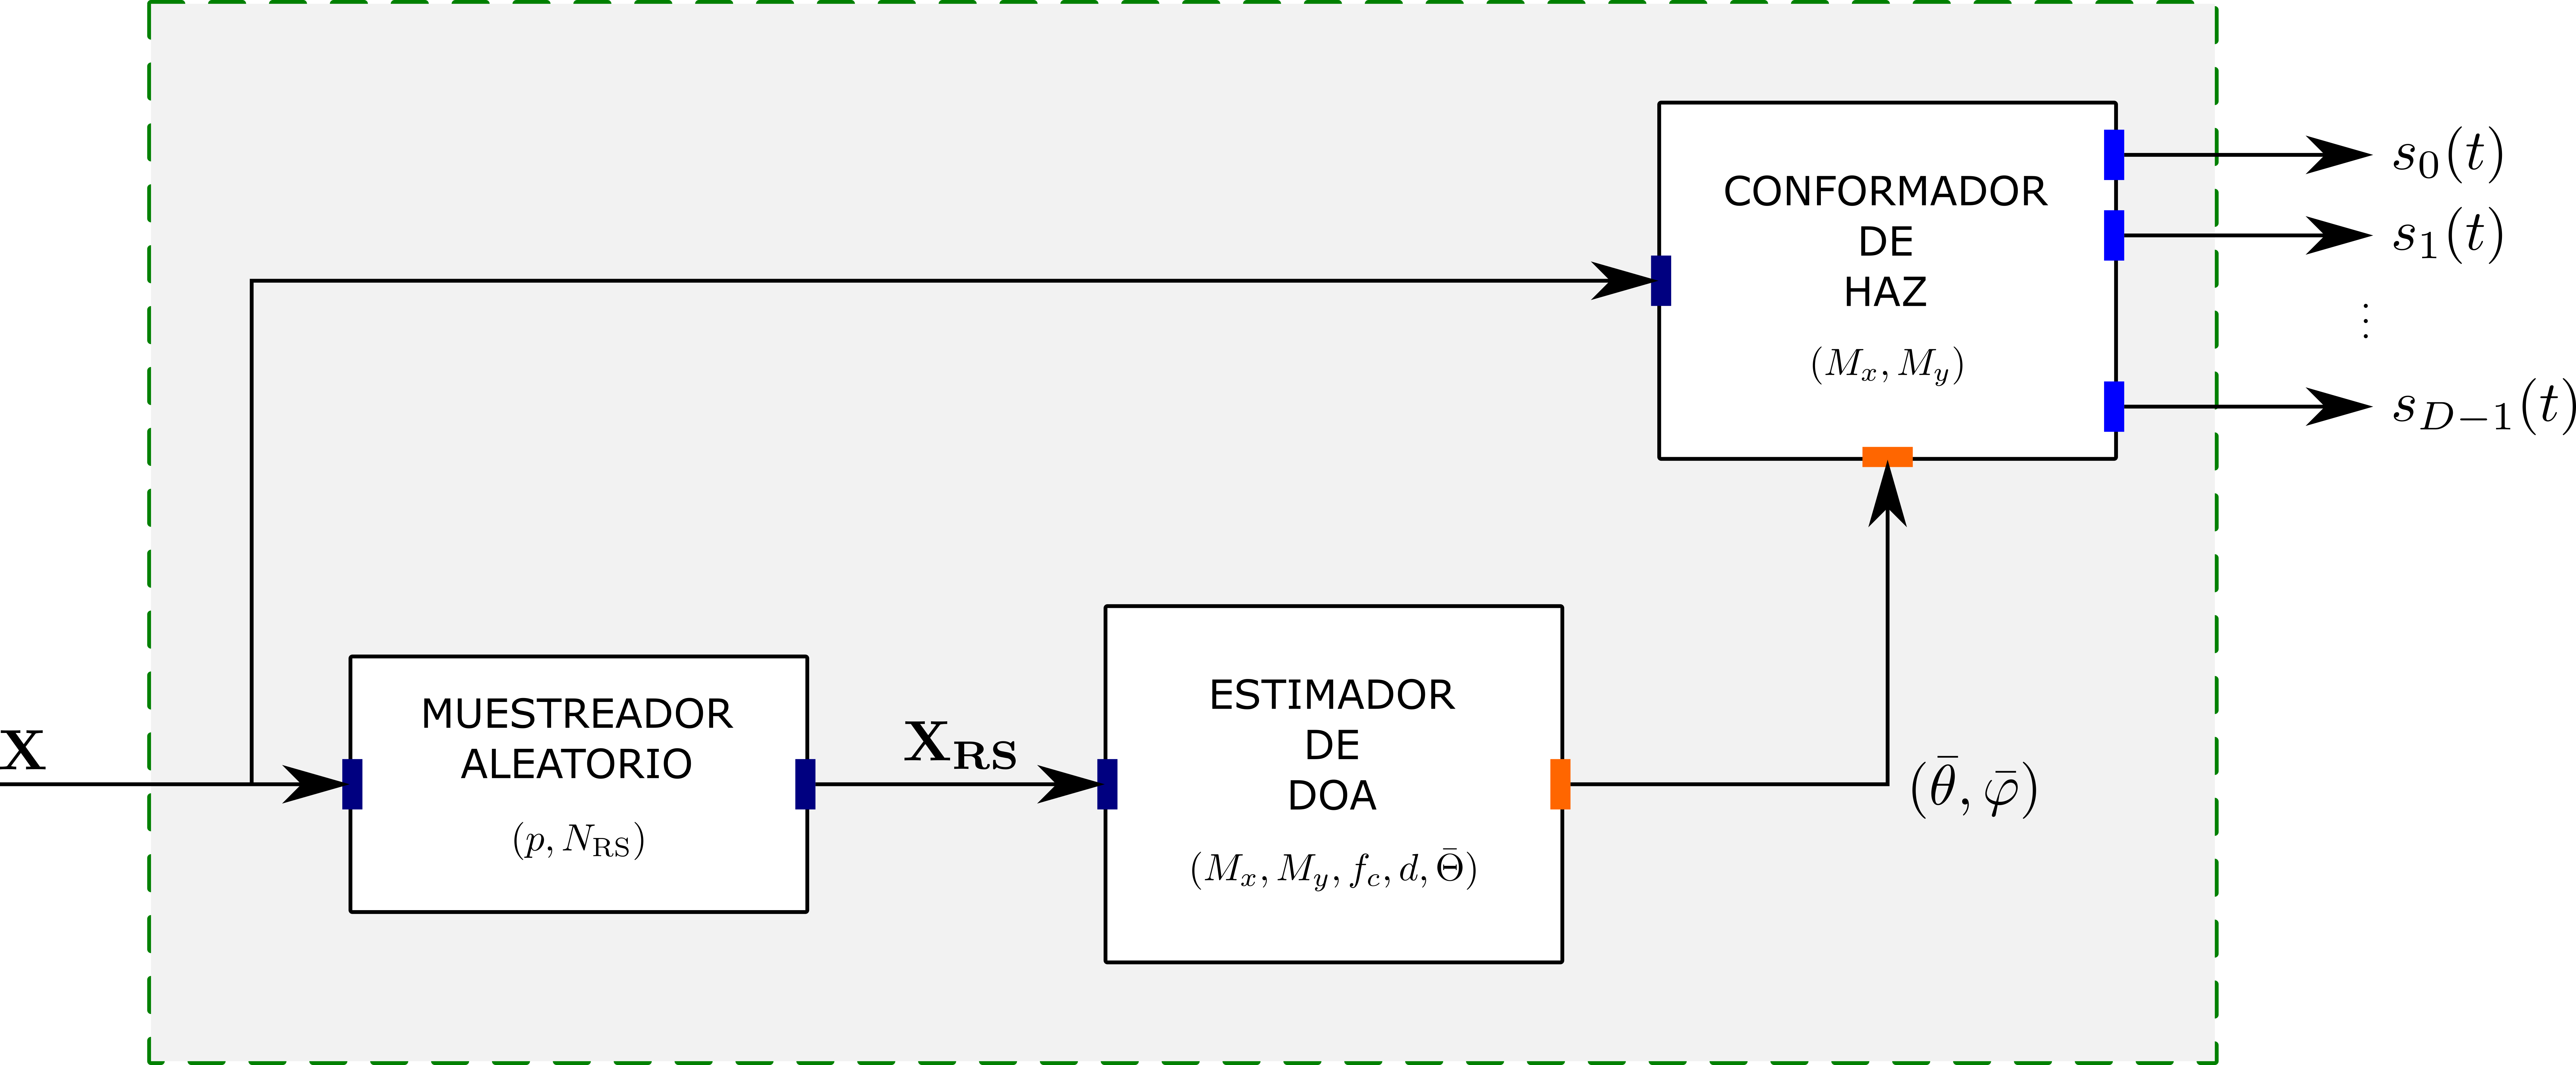
\includegraphics[width=0.9\linewidth]{images/06-Sistema/sistema_bd.png}
    \caption{Diagrama de bloques del sistema conformador de haz.}
    \label{fig:sistema_bd}
\end{figure}

Antes de operar el sistema debe ser configurado con los siguientes parámetros:
\begin{itemize}
    \item $M_x$: cantidad de elementos del arreglo de antenas en la dirección $x$.
    \item $M_y$: cantidad de elementos del arreglo de antenas en la dirección $y$.
    \item $f_c$: frecuencia nominal de portadora de las señales que se esperan recibir.
    \item $d$: distancia de separación entre elementos.
    \item $p$: probabilidad de tomar un vector de muestras en el muestreo aleatorio.
    \item $\bar{\Theta}:$ vector de parámetros del clasificador SVM obtenido mediante entrenamiento del algoritmo.
\end{itemize}

Este sistema puede ser implementado completamente en el PS, sin embargo la implementación de algunos de estos tres bloques en la FPGA puede llegar a traer alguna ganancia de rendimiento mediante la paralelización de cálculos, principalmente a medida que se aumenta la cantidad de señales recibidas, sin embargo al realizar esto se debe tener cuidado con las interfaces que se agregan entre el PS y la PL, ya que pueden llegar a ser un cuello de botella en el proceso, como así también hay que tener en cuenta la cantidad de recursos que quedan libres en la FPGA luego de que se instale el sistema de adquisición.

\section{Muestreador aleatorio}\label{subc:sistema_randomsampler}

El subsistema muestreador aleatorio recibe la matriz de muestras complejas $\mathbf{X}$ de tamaño $M \times N$ desde el sistema de adquisición y entrega una matriz de muestras $\mathbf{X_{RS}}$ de tamaño $M \times N_{\textrm{RS}}$ donde $N_{\textrm{RS}} = p\cdot N$. En este caso $p$ puede considerarse un factor de decimación, ya que es el número que define cómo se reduce la cantidad de muestras a la salida a partir de una cierta cantidad de muestras en la entrada. La matriz de salida se forma mediante elecciones aleatorias de las columnas de $\mathbf{X}$, utilizando el método que se explica en el Capítulo \ref{ch:randomsampling}.

\begin{figure}[ht!]
    \centering
    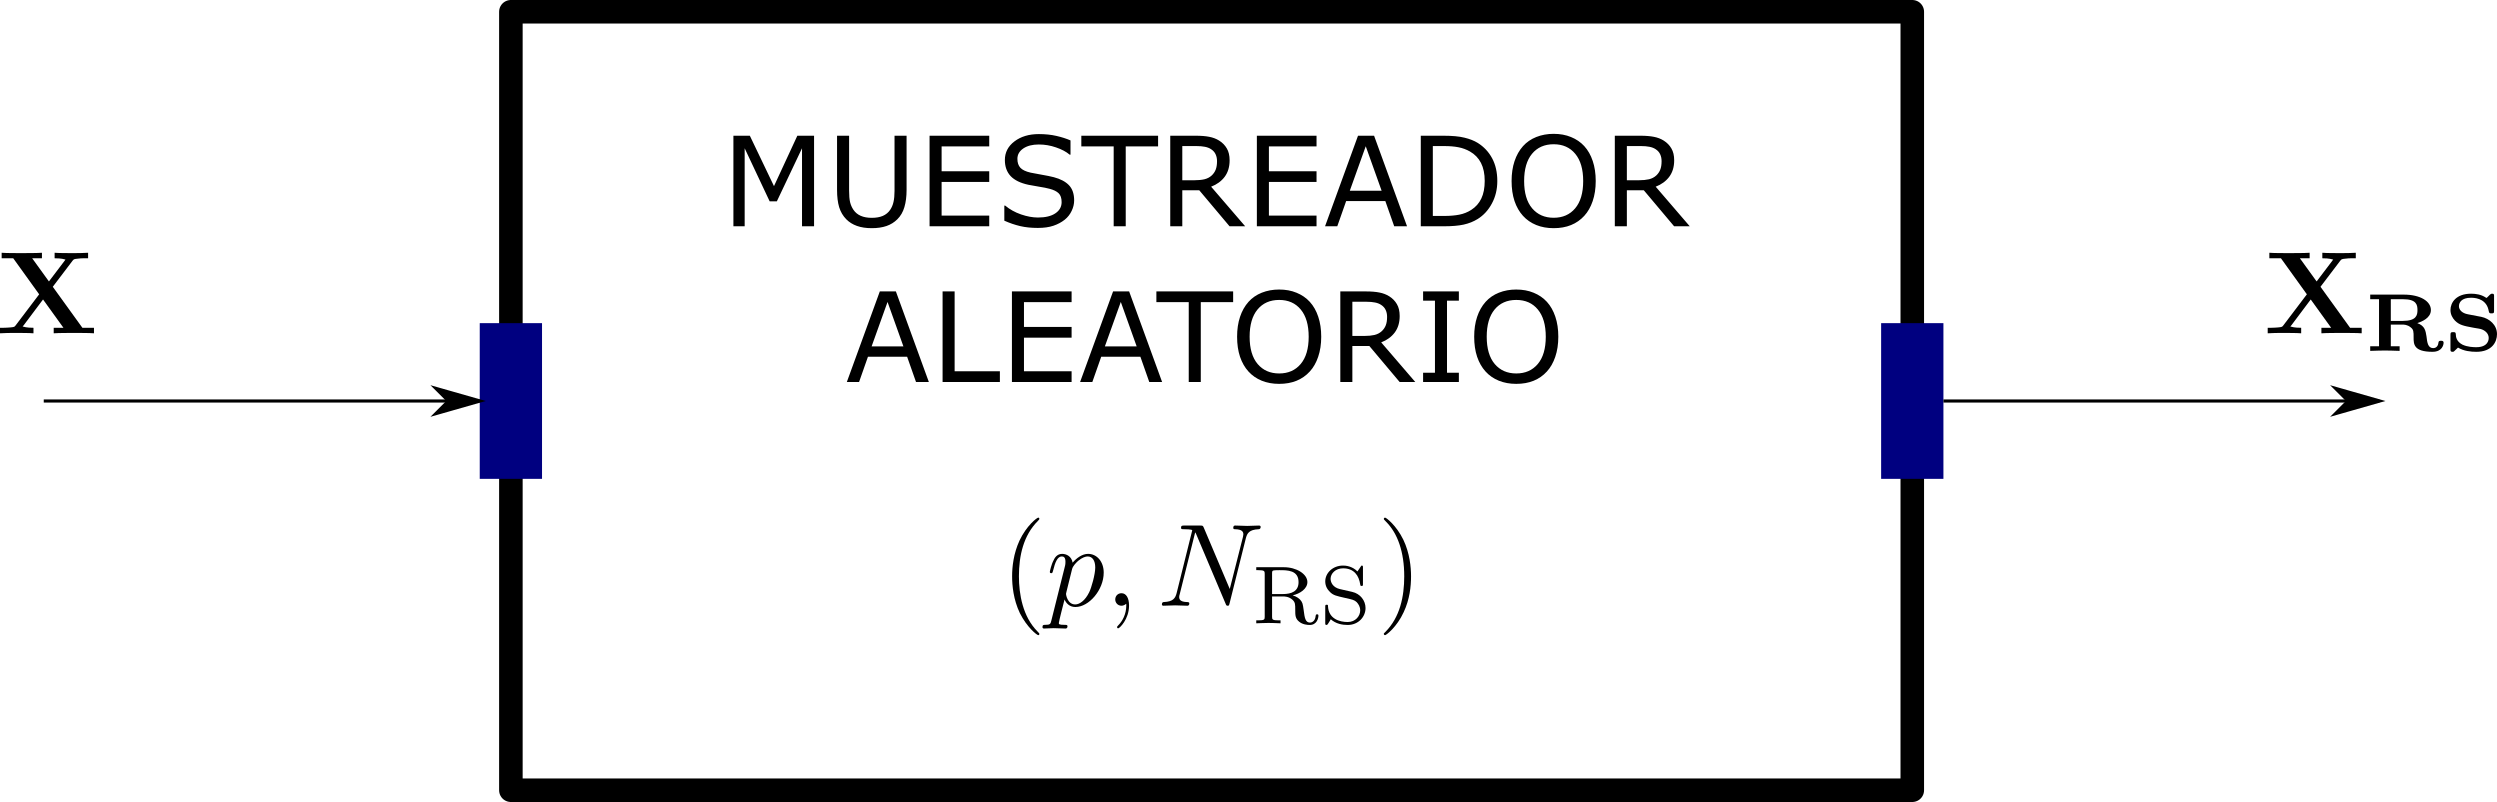
\includegraphics[width=0.6\linewidth]{images/06-Sistema/sistema_randomsampler.png}
    \caption{Representación en bloque del muestreador aleatorio con sus interfaces.}
    \label{fig:sistema_randomsampler}
\end{figure}

Otra manera de implementarlo es haciendo que este bloque reciba solo vectores de tamaño $M \times 1$ y que estos vectores se muestren en la salida con probabilidad $p$. Esta implementación evita tener que operar con matrices de tamaño $M \times N$.

\subsection{Implementación en FPGA}

Debido a que este módulo trabaja directamente con las muestras que entrega el sistema de adquisición, el contar con las muestras de cada elemento almacenadas en registros en la PL \cite{bib:jiqdc} permite una implementación rápida de este bloque que puede significar un ahorro de recursos en el PS, ya que, ubicando el muestreador aleatorio fuera del PS, se podría pensar en una implementación en el que este esté trabajando siempre con matrices de tamaño $M\times N_{\textrm{RS}}$ y no $M\times N$, reduciendo el consumo de memoria y los tiempos de carga de datos. A partir de esto, en la Figura \ref{fig:sistema_randomsampler_fpga} se muestra el diseño de bloques de una propuesta de implementación de este módulo en FPGA.

\begin{figure}[ht!]
    \centering
    \includegraphics[width=0.9\linewidth]{images/06-Sistema/sistema_randomsampler_fpga.png}
    \caption{Diseño de bloques de la propuesta de implementación del muestreador aleatorio en la FPGA.}
    \label{fig:sistema_randomsampler_fpga}
\end{figure}

Este diseño cuenta con 16 FIFOs \footnote{\emph{First in, first out}: bloque que permite el almacenamiento y la lectura de datos de manera tal que el primer dato en ser almacenado sea el primero en ser leído.}, una por cada elemento del ARU, capaces de almacenar una cantidad $N_{\textrm{RS}}$ de datos de 32 bits, suponiendo (sin pérdida de generalidad) que estos datos almacenan la parte real y la parte imaginaria de una muestra en porciones de 16 bits para cada una. Cada FIFO tiene una señal \texttt{FULL} que sirve para indicar al subsistema estimador de DOA el momento en el que las muestras se encuentran listas para ser procesadas, instante en el cual este subsistema puede levantar la señal de lectura para comenzar con la carga de los datos. La escritura de las FIFOs se realiza simultáneamente a partir de una señal externa que indica cuándo existen datos válidos en las entradas, y una señal interna generada a partir de la comparación de dos números de 16 bits: el número $p$ fijado por el usuario y otro número generado aleatoriamente cada tiempo de reloj por un bloque generador de números aleatorios. De esta manera, las FIFOs se cargan en tiempos aleatorios pero de manera simultánea entre ellas, entregando en sus salidas en el momento de lectura los vectores de la matriz $\mathbf{X_{RS}}$ que se muestra en la Figura \ref{fig:sistema_randomsampler}. En este caso no se utiliza la señal de \texttt{EMPTY} de las FIFOs ni se evita la escritura en las mismas cuando la señal \texttt{FULL} se encuentra en alto debido a que se busca que las FIFOs se encuentren actualizadas en todo momento con las muestras más recientes, ya que en esas muestras se encontrará la información de la DOA, la cual se desea mantener siempre actualizada. El único momento en el cual se debe impedir la escritura de datos es el momento en el que el subsistema estimador de DOA se encuentra haciendo la lectura de los datos que se encuentran dentro de las FIFOs.

\section{Estimador de dirección de arribo}\label{subc:sistema_doa_estimator}

El subsistema estimador de dirección de arribo, cuya representación como bloque se muestra en la Figura \ref{fig:sistema_doaest}, es el subsistema más complejo de los tres debido a las operaciones que realiza. Como se muestra en la Figura \ref{fig:sistema_doaest_2}, está conformado por 3 bloques:

\begin{itemize}
    \item \textbf{SVD:} bloque encargado de realizar la descomposición en valores singulares de la matriz de entrada $\mathbf{X_{RS}}$, obteniendo la matriz de valores singulares $\mathbf{\Sigma}$ y los vectores singulares izquierdos $\mathbf{E}$.
    \item \textbf{SVM:} bloque encargado de realizar la estimación de la cantidad de señales recibidas $D$ realizando una clasificación de los valores singulares contenidos en la matriz $\mathbf{\Sigma}$ utilizando el algoritmo de Máquina de Vectores de Soporte que se analizó en la Sección \ref{subc:ml_svm}. Utilizando un kernel gaussiano, el vector $\bar{\Theta}$ debe incluir, además, los parámetros adicionales $C$ y $\gamma$.
    \item \textbf{ESPRIT:} bloque encargado de realizar la estimación de DOA de las $D$ señales recibidas a partir de los vectores singulares izquierdos de la matriz $\mathbf{E}$. En su salida entrega los vectores $\bar{\theta}$ y $\bar{\varphi}$ de tamaño $D\times 1$.
\end{itemize}

Debido a la dinámica en el tamaño de los datos con los que opera este subsistema, ya que un cambio en la cantidad de señales recibidas implica un cambio en la cantidad de columnas con las que debe operar el bloque ESPRIT, y a la dificultad de implementar los algoritmos algebraicos de los bloques SVD y SVM en FPGA, comparada con la escasa dificultad de implementarlos en software, este sistema debe ubicarse en el PS.
\begin{figure}[ht!]
    \centering
    \begin{subfigure}[b]{0.5\textwidth}
        \centering
        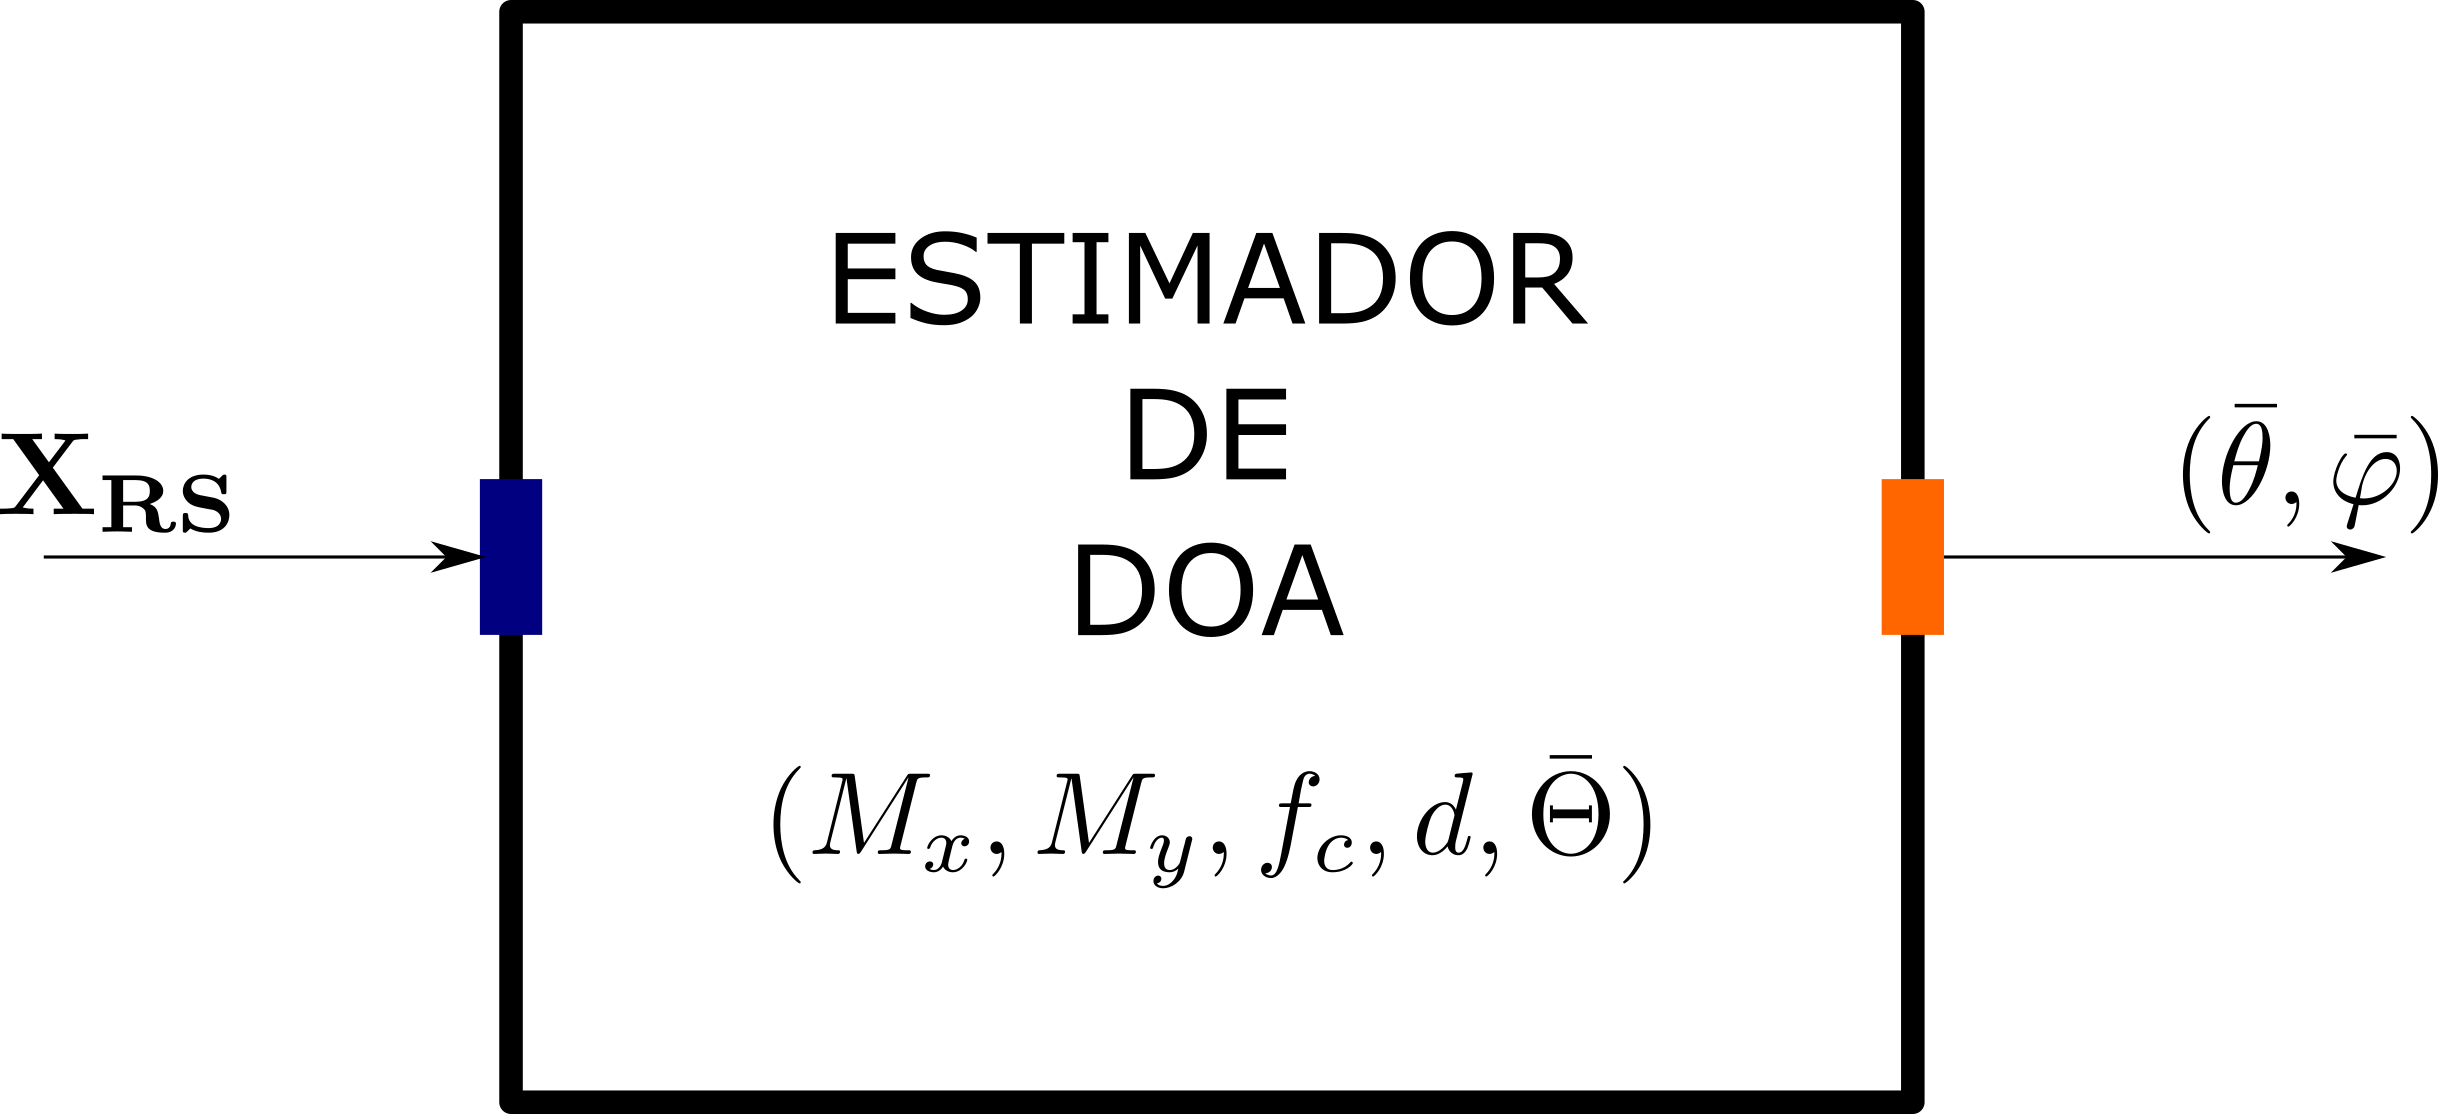
\includegraphics[width=\linewidth]{images/06-Sistema/sistema_doaest.png}
        \caption{Bloque.}
        \label{fig:sistema_doaest}
    \end{subfigure}
    \hfill
    \begin{subfigure}[b]{0.9\textwidth}
        \centering
        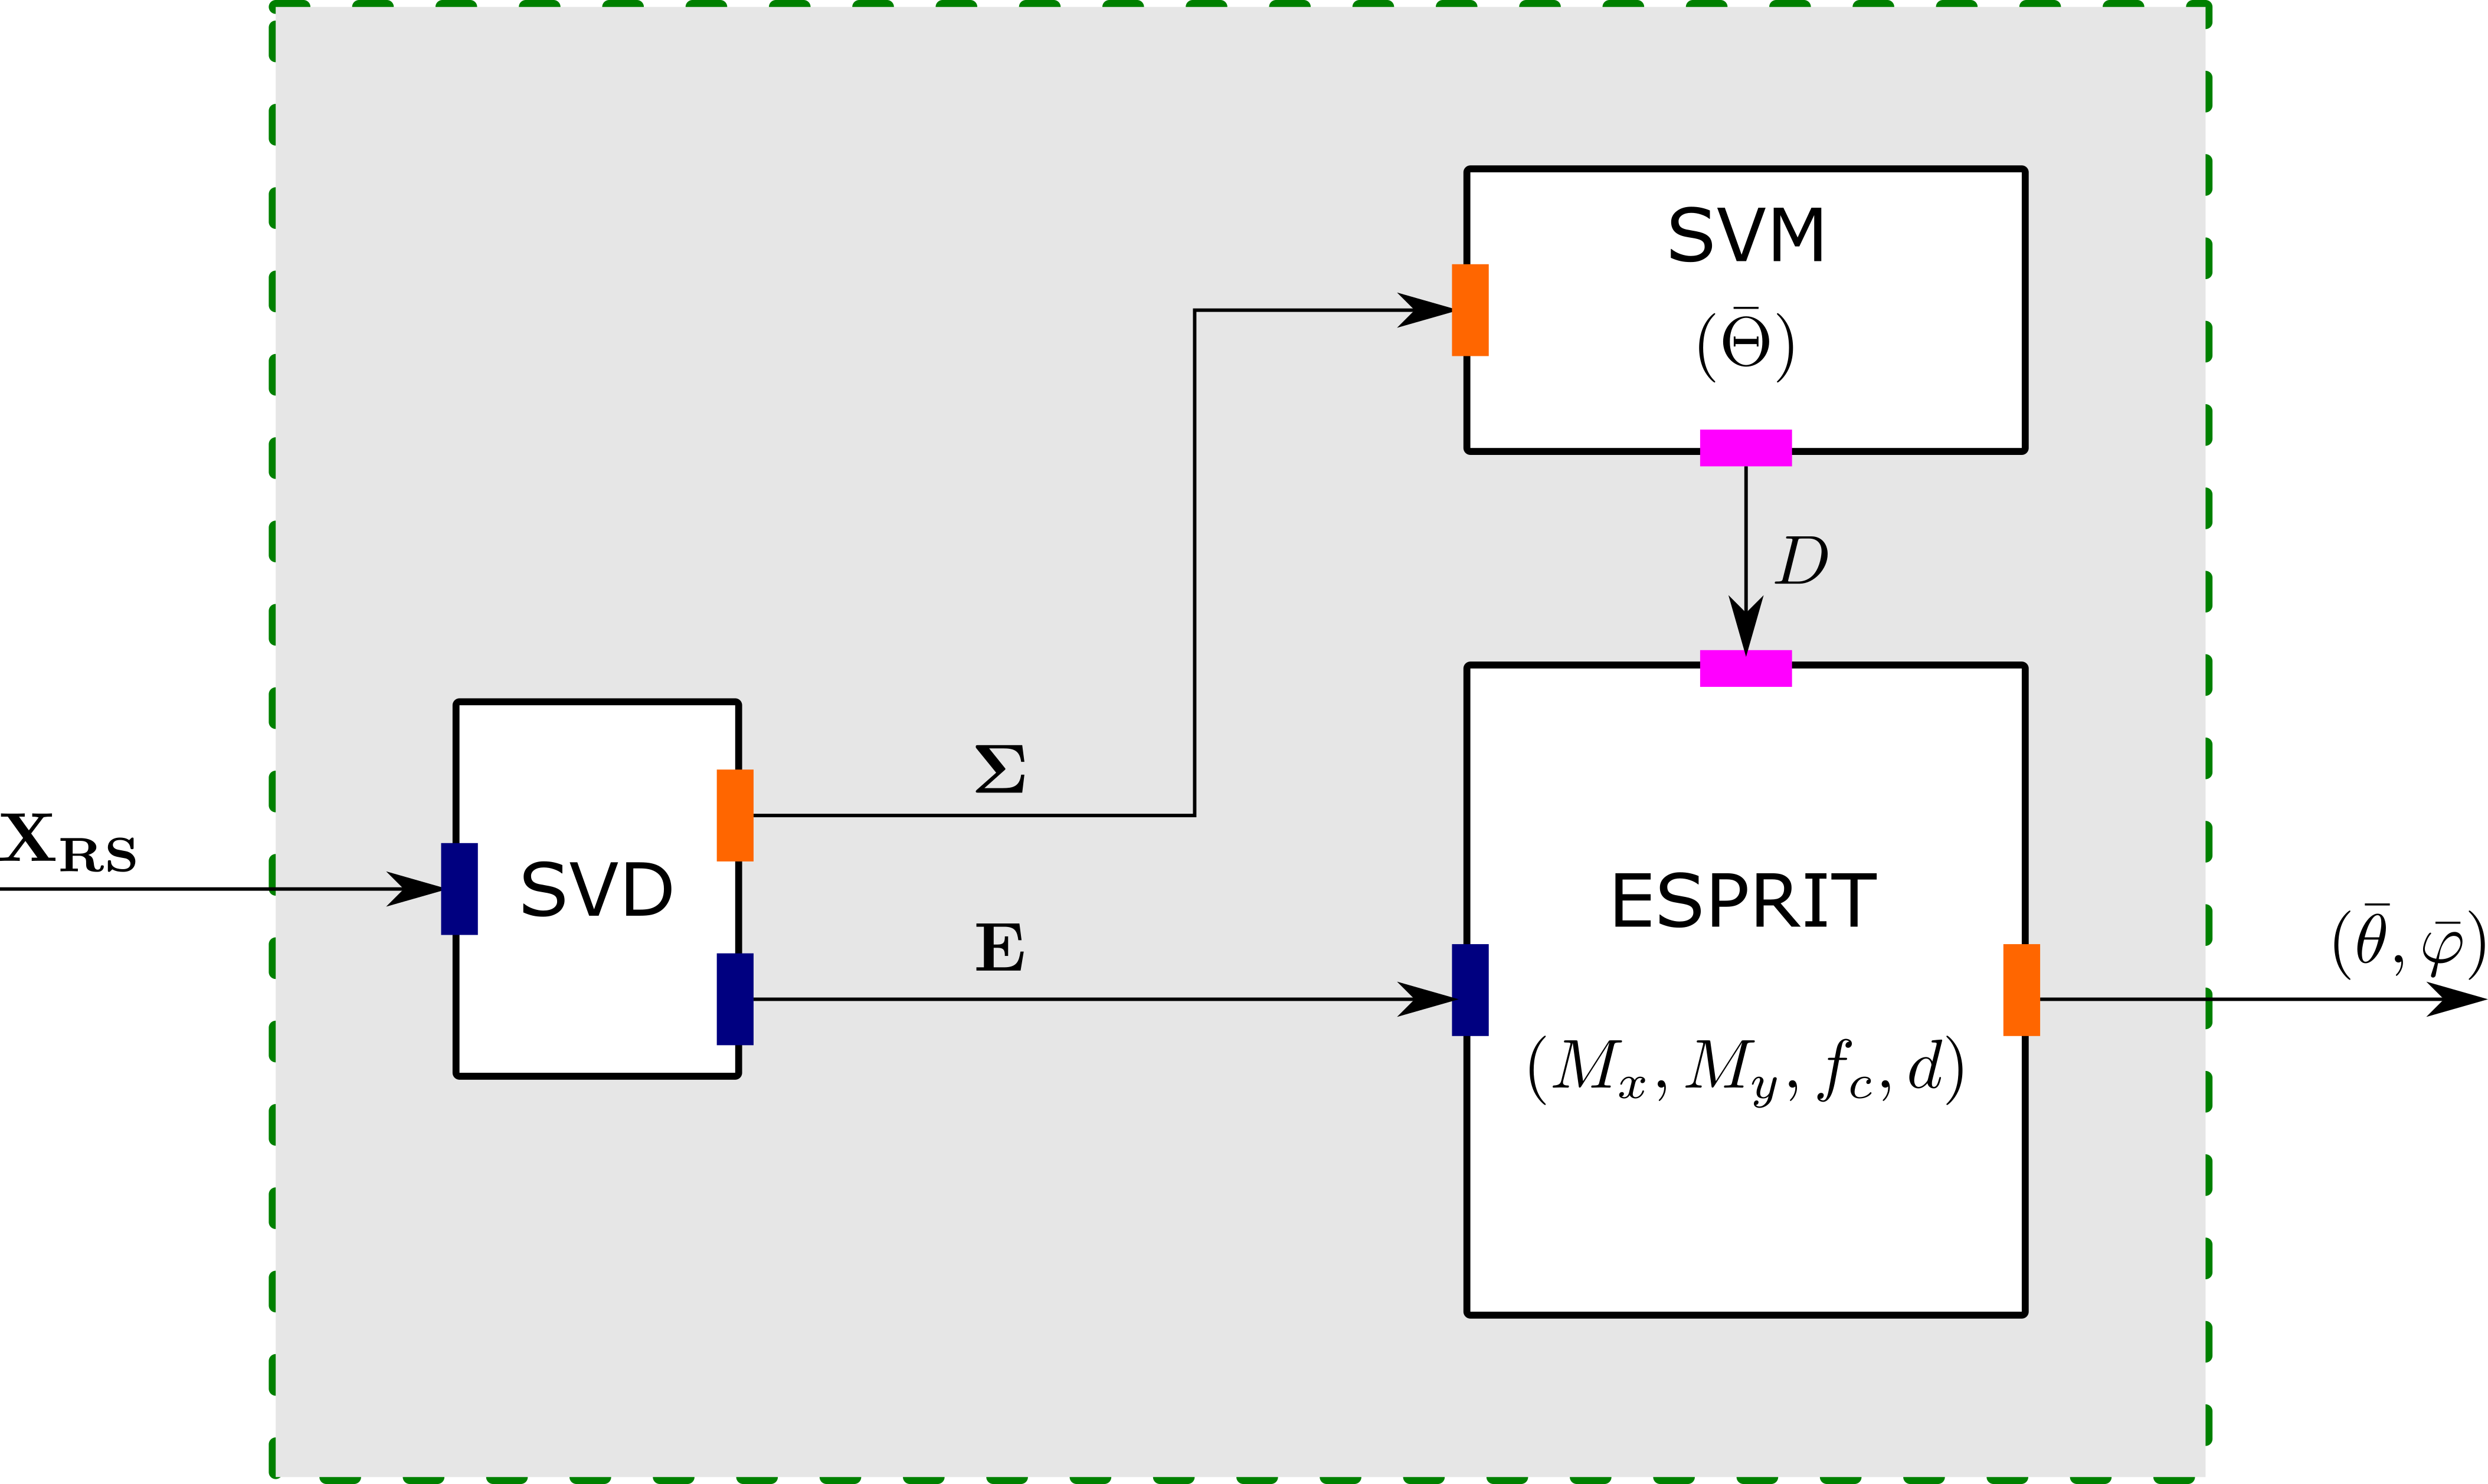
\includegraphics[width=\linewidth]{images/06-Sistema/sistema_doaest_2.png}
        \caption{Detalle del subsistema.}
        \label{fig:sistema_doaest_2}
    \end{subfigure}
    \caption{Representación como bloque del subsistema estimador de DOA con sus correspondientes interfaces.}
\end{figure}



\section{Conformador de haz}\label{subc:sistema_beamformer}

El último subsistema a implementar es el conformador de haz, cuya representación en bloque se muestra en la Figura \ref{fig:sistema_beamformer}. Con la información obtenida de los otros dos subsistemas, el conformador de haz se encarga de procesar las muestras de cada elemento del ARU restándole la diferencia de fase con respecto al elemento de referencia y promediando todas las muestras de manera tal de obtener las $D$ señales a la salidas. Además, si se conoce el patrón de radiación de cada elemento del ARU puede afectarse a cada muestra por la ganancia del arreglo en la DOA para normalizar las señales recibidas. Por cada señal detectada la operación que realiza este subsistema es la siguiente:

\begin{align}
    \hat{s_d}[n] & =\frac{1}{M\left(g(\hat{\theta}_d,\hat{\varphi}_d)\right)^2}\cdot\bar{a}_{\textrm{ARU}}^H(\hat{\theta}_d,\hat{\varphi}_d) \cdot \bar{x} \\
                 & =\frac{1}{M\cdot g(\hat{\theta}_d,\hat{\varphi}_d)} \cdot \begin{bmatrix}
        1 & \cdots & e^{jkd[(M_x-1)\cos \hat{\theta}_d \cos \hat{\varphi}_d+(M_y-1)\cos \hat{\theta_d} \sin \hat{\varphi}_d]}
    \end{bmatrix} \cdot \begin{bmatrix}
        x_0 \\
        x_1 \\
        x_{M-1}
    \end{bmatrix}    \nonumber      \\
                 & = \frac{1}{M\cdot g(\hat{\theta}_d,\hat{\varphi}_d)} \sum_{m=0}^{M-1} a_m^*(\hat{\theta}_d,\hat{\varphi}_d) \cdot x_m,\nonumber
\end{align}
con $d=0,1,...,D-1$ y donde $\bar{a}_{\textrm{ARU}}$ es el vector de apuntamiento definido en la Ecuación \ref{eq:beamforming_a_aru}

\begin{figure}[ht!]
    \centering
    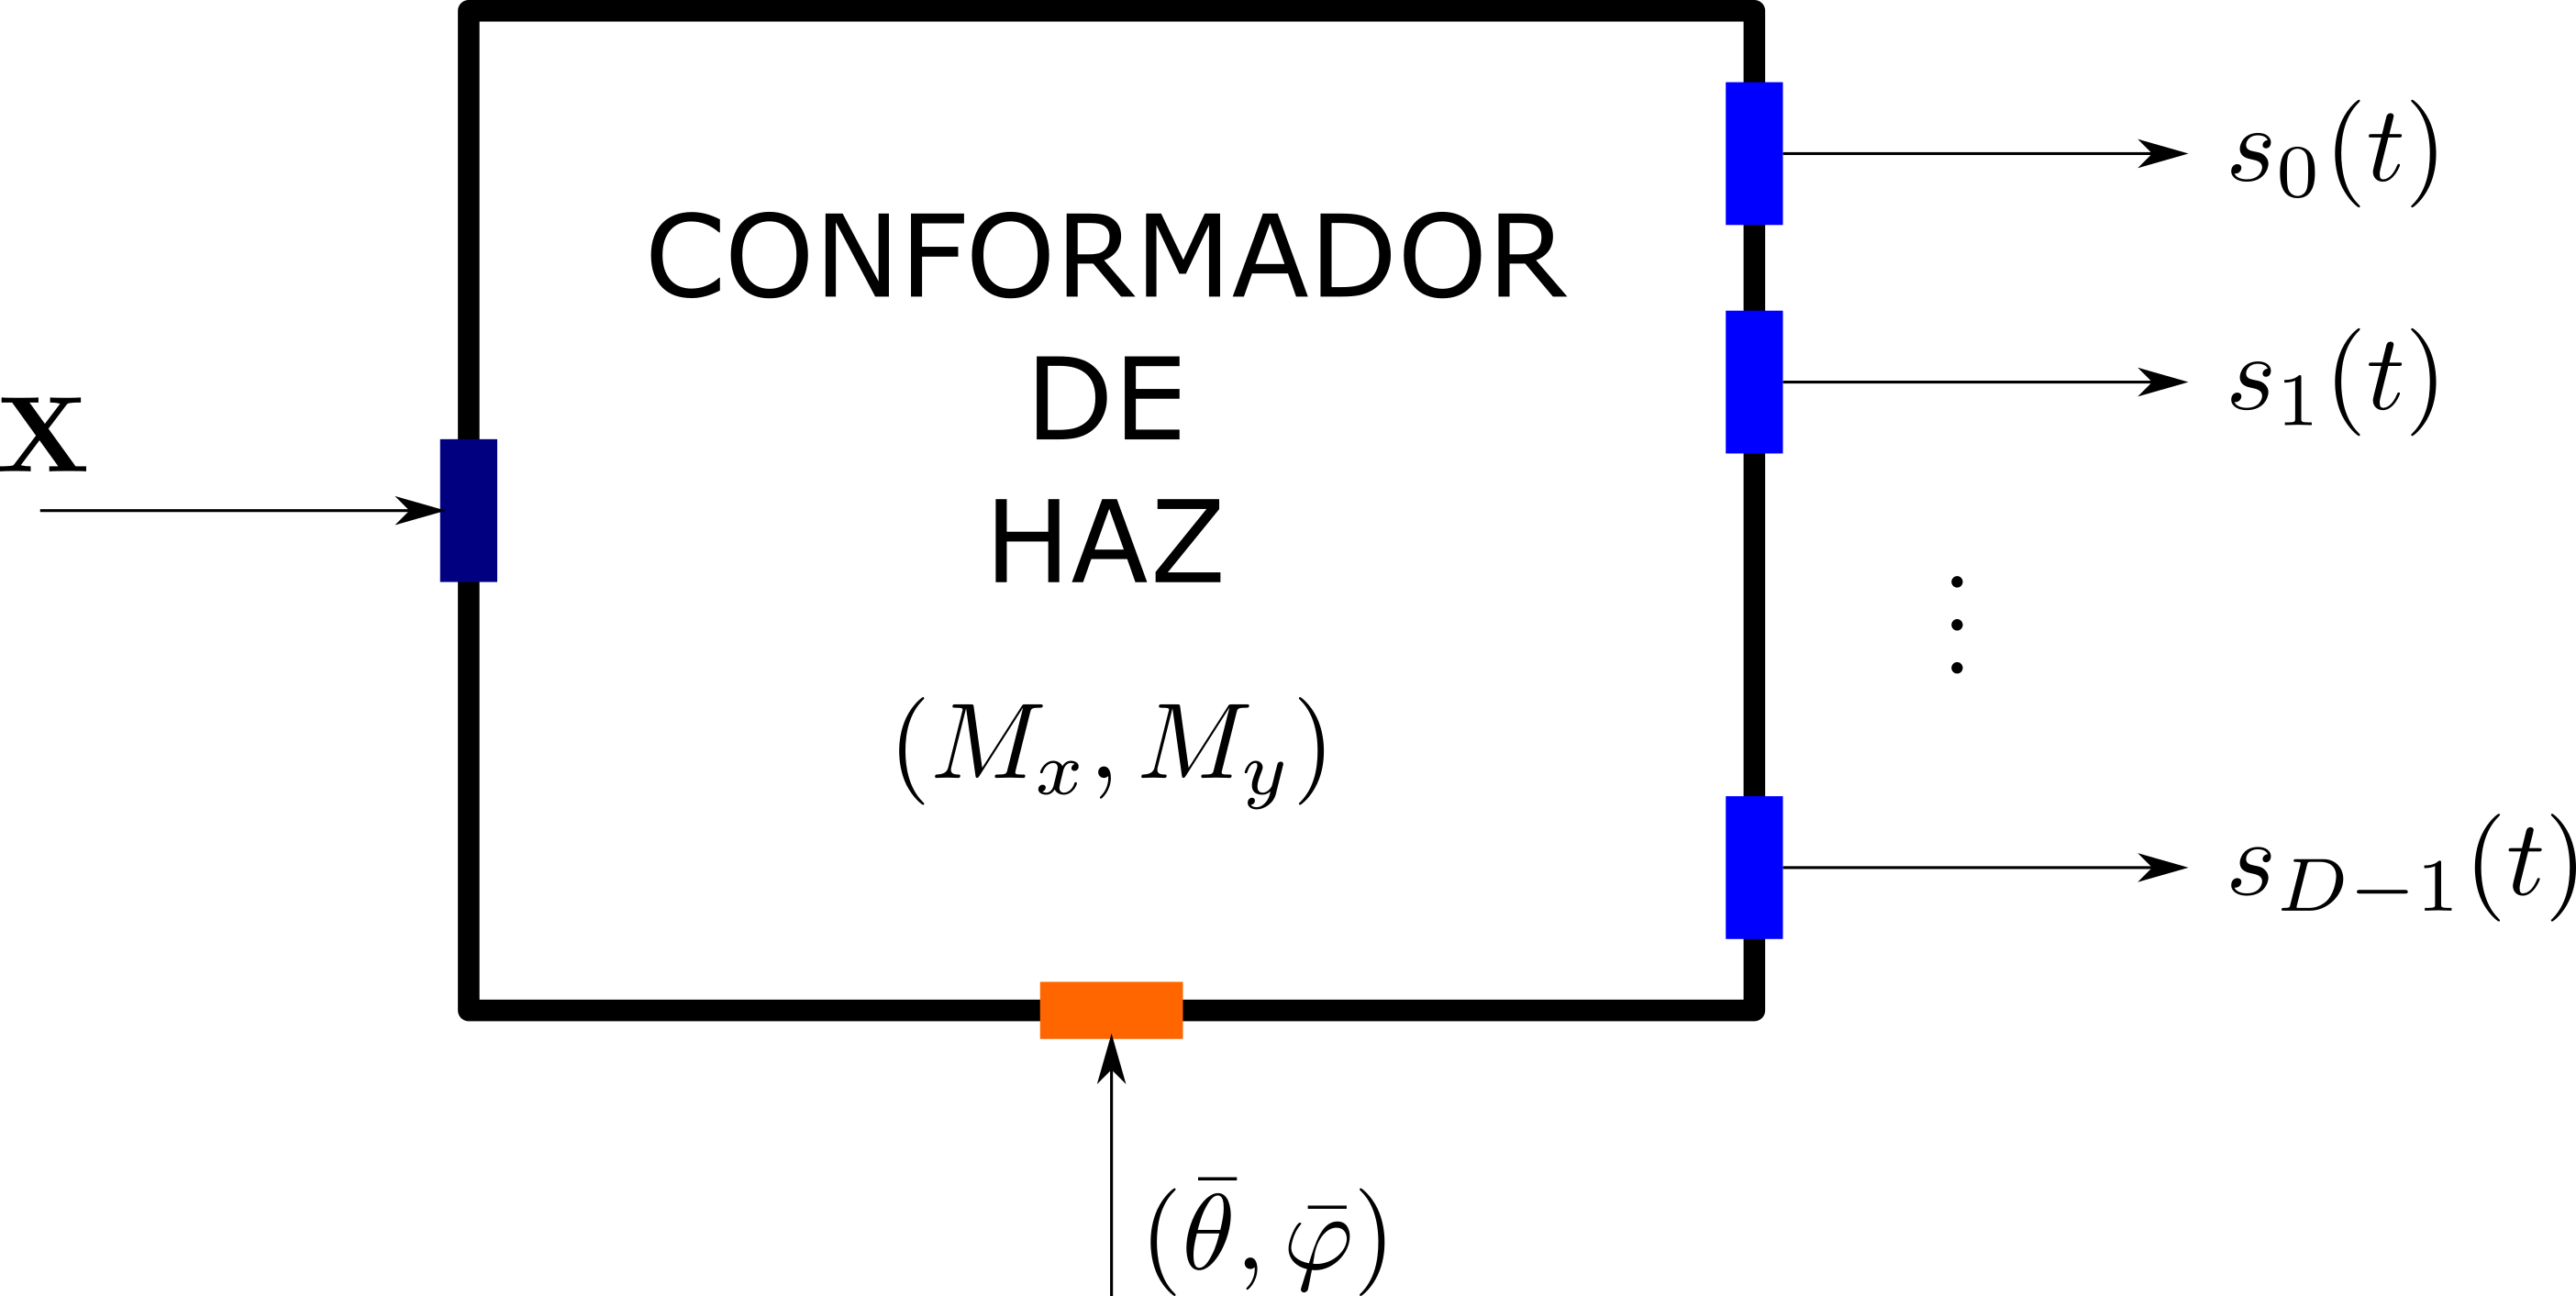
\includegraphics[width=0.5\linewidth]{images/06-Sistema/sistema_beamformer.png}
    \caption{Representación como bloque del subsistema conformador de haz con sus correspondientes interfaces.}
    \label{fig:sistema_beamformer}
\end{figure}

\subsection{Implementación en FPGA}

Este algoritmo puede ser implementado tanto en el PS como en la FPGA, debido a que no requiere realizar cálculos de mayor complejidad. Una ventaja de implementarlo en la PL junto al muestreador aleatorio es, como ya se mencionó, evitar que el PS tenga que manipular matrices de tamaño $M\times N$ y en su lugar trabajar con matrices $M\times N_{\textrm{RS}}$ donde $N_{\textrm{RS}}$ puede ser incluso más de dos órdenes de magnitud menor que $N$. En la Figura \ref{fig:sistema_beamformer_fpga} se muestra un diagrama de bloques de una propuesta de implementación de este subsistema en FPGA.

\begin{figure}[ht!]
    \centering
    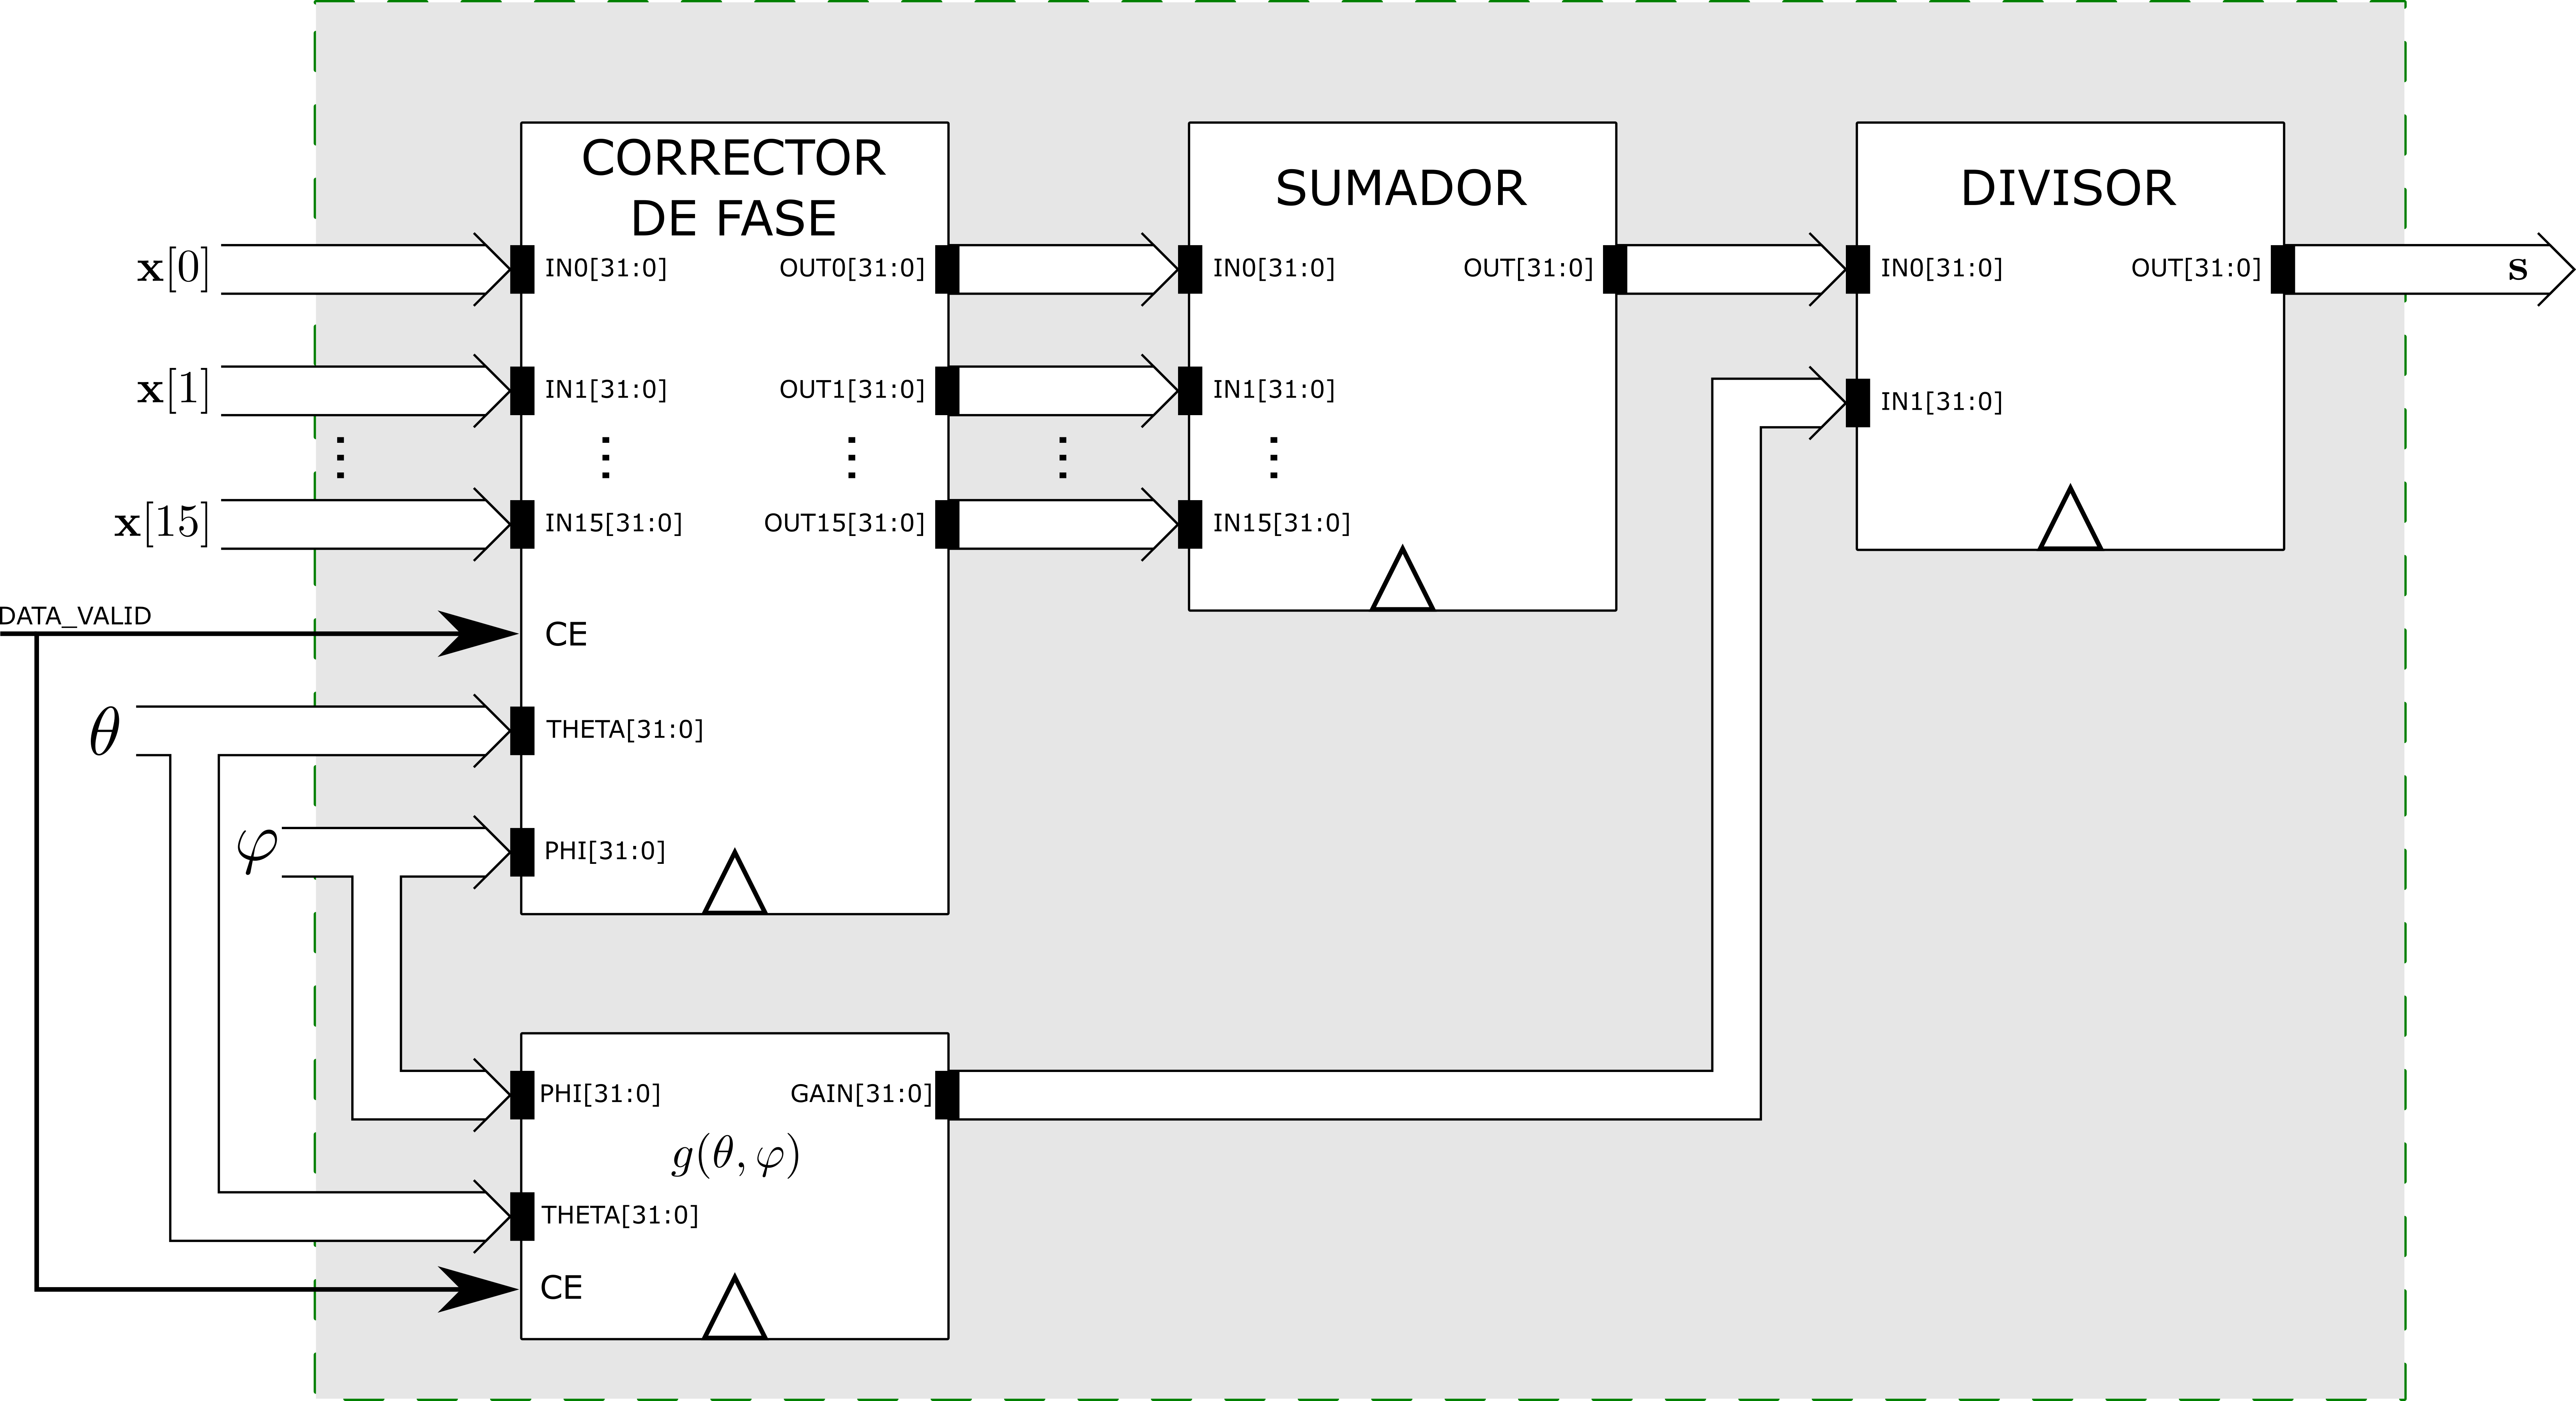
\includegraphics[width=0.9\linewidth]{images/06-Sistema/sistema_beamformer_fpga.png}
    \caption{Propuesta de implementación del subsistema conformador de haz en FPGA.}
    \label{fig:sistema_beamformer_fpga}
\end{figure}

En este diseño el sistema recibe como entradas las 16 muestras de 32 bits provenientes del sistema de adquisición, los ángulos de elevación y azimut provenientes del subsistema estimador de DOA (el cual se encuentra en el PS), y una señal de validación proveniente del PS que indica el instante en el que existen ángulos de arribo válidos en las correspondientes entradas. Dentro del subsistema existen cuatro bloques: un corrector de fase, el cual se encarga de restar la fase de cada muestra dependiendo de con qué elemento fue tomada, un bloque sumador que suma las 16 salidas del bloque corrector de fase para realizar el promediado de la señal recibida, un bloque que a partir de una DOA entrega la ganancia del ARU en esa dirección, y un divisor que utiliza esta ganancia para normalizar la señal recibida. Siendo que en este caso la cantidad de elementos del ARU es 16, el promediado puede hacerse quitando los 4 bits menos significativos de esta salida. Hay que notar que este diseño solo sirve para realizar la conformación de haz de una única señal, en caso de aumentar las salidas del sistema debe repetirse este bloque y alimentarlo con las direcciones de arribo de las señales restantes. Esta es una desventaja de la implementación en la PL, ya que el diseño no puede ser dinámico según la información recibida y debe ser dimensionado para el peor caso.